\chapter{Material and Methods}

\section{Data sets}

\section{Algorithms}

describe MaxEnt, NB, SVM, Boosting/Bagging


\chapter{Experimental Setup}
\label{sec:experimentalsetup}

\section{Architecture}

This section describes the overall architecture and how the system works. First the general system will be described, and then the API Layer and classification server in turn.  

To make the system as modularized and responsive as possible, the API layer was written in Node.js and the sentiment classifier in the Python programming language. Both systems are continuously running servers. This allows multiple services to run simultaneously, both for the API layer and the classifier. The idea is to make the system horizontally scalable.

\begin{figure}[ht]
 \begin{center}
     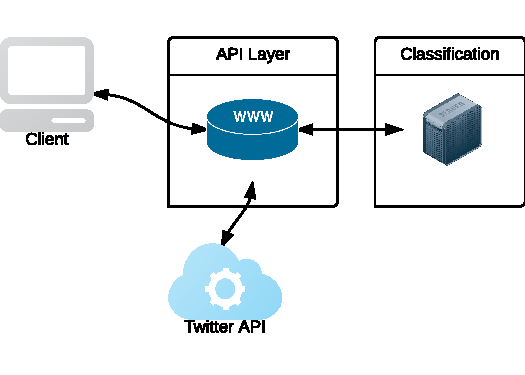
\includegraphics[width=0.8\textwidth]{../img/NetworkDiagram.pdf}
 \end{center}
 \caption[Architectural overview of the system.]{Architectural overview of the system. The client retrieves data from the Twitter API and uses the classification server for sentiment classification.}
 \label{fig:NetworkDiagram.pdf}
\end{figure}

A client makes a request to the API Layer, with the same interface as the Twitter API service. From there the API Layer will retrieve information from the Twitter API with HTTP requests, iterate over all tweets received, and send them in parallel to the classification server. When the classification server is done processing and classifying the tweet, it is sent back to the API Layer. When the API layer has received all the tweets, it responds to the client with the same JSON structure as the Twitter API sends out, only with an additional attribute noting the tweet's sentiment. This architecture and application flow can be seen in~\autoref{fig:NetworkDiagram.pdf}. 

\subsection{API Layer Extension}

To be able to have a scalable and responsive solution, the API Layer was written using the Node.js platform. Since Node.js uses JavaScript as programming language, the JSON data retrieved from the Twitter REST and Streaming API are easily manipulated and passed around. 

The API Layer works as a thin layer extending the Twitter API. This means that the interface used by Twitter, with all defined options and appropriate methods, is reflected through the API Layer. The main benefit is that all documentation for the Twitter API also documents most of this extended API Layer.

For authentication, an application is registered with a developer account at the Twitter Developer site. This creates OAuth credentials, which is used to identify the application, and to gain access to the Twitter data. For this implementation, the data is retrieved using the OAuth access for the application, not at user level. 

\subsubsection{Architectural Flow}


\begin{figure}[htb]
 \begin{center}
     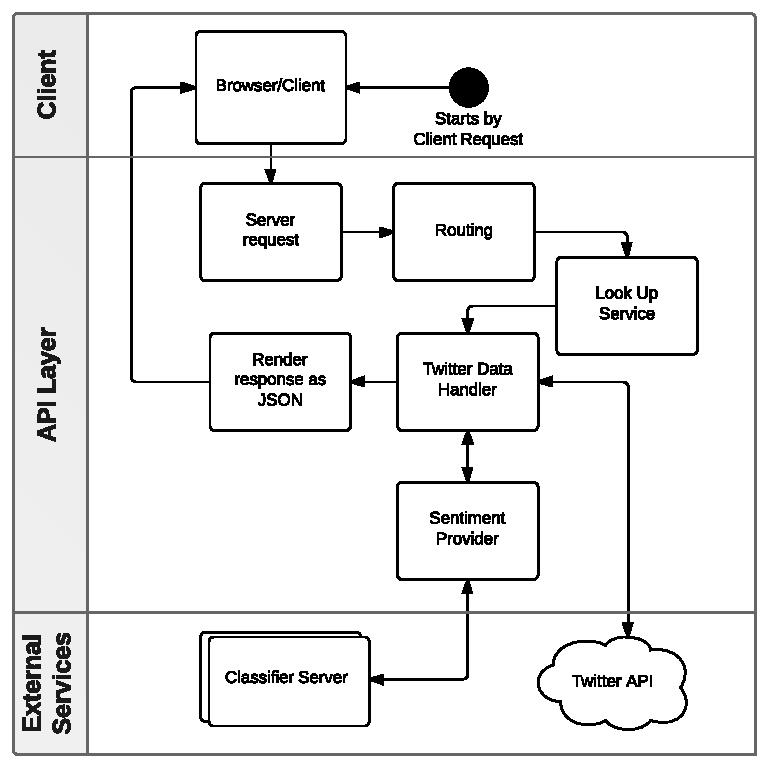
\includegraphics[width=0.8\textwidth]{../img/APILayerArcitechture.pdf}
 \end{center}
 \caption[Architectural overview of the API Layer.]{Architectural overview of the API Layer. A request is handled by the server, sending it to routing where it is processed and sent to service look-up. If a service is found, a request is sent to the Twitter API and the received data is extended by the Twitter Data Handler module to contain a sentiment. When all of the Twitter data are extended, the data is given as a response to the requesting client.}
 \label{fig:APILayerArcitechture.pdf}
\end{figure}

When a request from a client is made, the request gets processed by the server and the routing module determines what the client is looking for. When the proper service is found, the client-specified parameters are sent directly to the Twitter API, using the Twitter Data Handler module (TDH). The TDH module then iterates over all found tweets, and sends them in parallel to the classification server. When a tweet has been processed by the classification server the classified sentiment is sent back to the TBH module and the original tweet object is extended to contain a property with the sentiment. When all tweets are classified, the TBH module passes the extended twitter data to the render module. The render module renders the JSON data and sends it to the client with appropriate HTTP headers set. This application flow can be seen in~\autoref{fig:APILayerArcitechture.pdf}.

If there is an error during any part of the process, the error is caught by the routing module, and the error is rendered as a JSON object, in the same manner as it would be by the Twitter API. 

When using both the Twitter REST API and Streaming API, there is a high level of asynchronism. Especially when streaming, it is impossible to predict when the next tweet is received. Due to this the system designed needs to be able to handle this dynamic data flow. Node.js is an event-driven platform and has a natural support for asynchronous data. 

All internal and external message passing in the API Layer is asynchronous. When requesting Twitter for data, an event is triggered when that data is ready and all tweets are separately sent to the classifier. By sending all tweets separately in parallel, classification of the entire set of tweets does not take much longer than classifying only one tweet. 

When streaming, the TBH module opens a connection to the Twitter API, but never closes it. There is a continuously open connection to the Twitter server, which is feeding the TBH module with single tweets as they get stored in the Twitter system. From the first received tweet, a connection to the requesting client is opened by the render response module. This connection will also remain open. In this way there is an open connection between the client and the API Layer as well as between the API Layer and the Twitter API. The API Layer works as a middleman, taking in tweets, classifying them, and streaming them to the client. By running this entire process asynchronously, the system can process data independently of when it is published.


\subsection{Sentiment Analysis Classifier}
\label{sec:classifier_arch}

Python is computationally stronger than Node.js in many ways. Additionally, it is much more mature. There are a lot of well documented packages for handling various tasks. Scikit-learn (sklearn) is one of these packages. sklearn is package built on top of the Python packages numpy, scipy and matplotlib. sklearn integrates machine learning algorithms as SVM, NB, MaxEnt and more. sklearn implements solutions for doing feature extraction, grid searching, cross validation and a lot more for analysing text. Thus it is a good choice for the process of sentiment analysis. As a dynamic typed language, Python allows for rapid development and prototyping. These attributes are some of the reasons Python is a good fit for the present system. 

The Sentiment Analysis Classifier system runs as a server waiting for requests. The HTTP method POST is used for a client to send a \textit{stringified} tweet object to the server. Stringify is a JSON method for returning a serialized object represented by a string. The classification server converts this string to a Python dictionary. The response will be a string with the sentiment classification, that is, either \textit{positive}, \textit{neutral} or \textit{negative}. The classification scheme can be extended if necessary. 

The classifier server can be initialized with different settings for classification strategy, what port to run at, what training data to use, and whether or not to show debug data. This allows for multiple servers running at the same time, with different settings. Running multiple server instances makes it easier to compare different classification strategies. Two servers could run side by side, and a test framework could use the two servers to classify the same tweets for a comparison.

When the server is initiated, the selected model is trained by having and made availeble to be used by the classification server. 

The classification server uses a pool of child processes. For each receiving tweet, it spawns a new child from this pool and in this process the tweet is classified. This way the classification server can process several tweets in parallel, which helps the one-to-one relationship between a tweet on the classification server and the same tweet on the API Layer.

\subsubsection{Architectural Flow}

\begin{figure}[htb]
 \begin{center}
     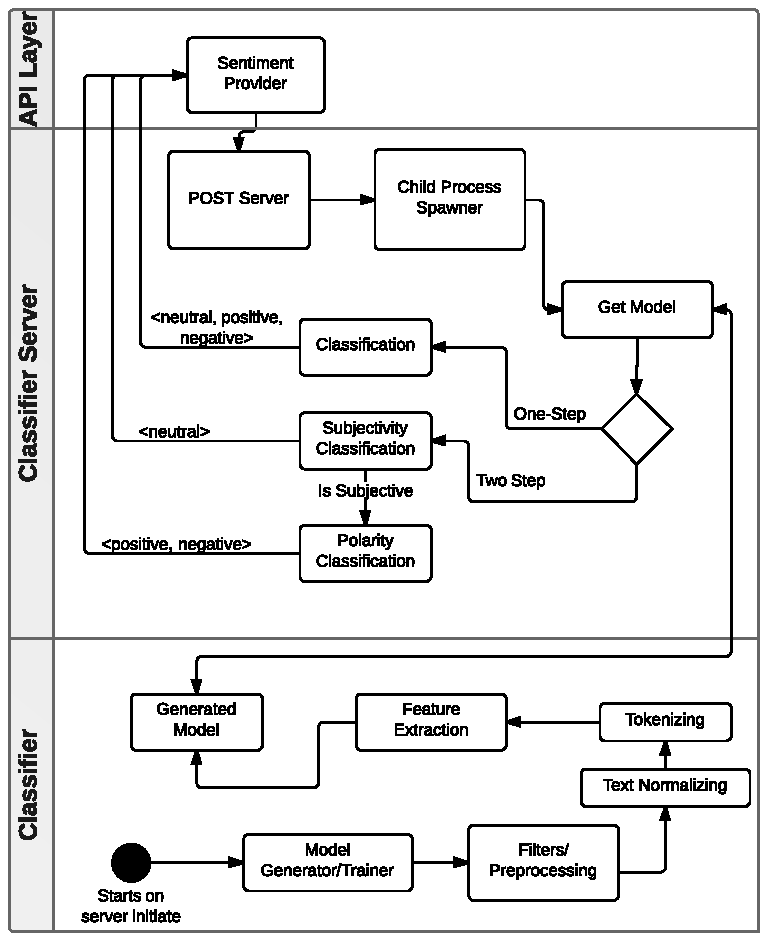
\includegraphics[width=0.8\textwidth]{../img/ClassifierArcitechture30.pdf}
 \end{center}
 \caption[Architectural overview of the classification server.]{Architectural overview of the classification server. On server start, a model for predicting seniment is generated. When a request from the API Layer is made to the POST Server, a child processes is spawned. The tweet text is extracted and sent into the model for classification. If the classification model is a one-step process, the classifier returns to the sentiment provider with either a neutral, positive or negative classification. If the generated model is two-stepped, the tweet is first classified as either neutral or subjective. If it is neutral, it is returned to the API Layer, if it is subjective, it is sent to the next step and the result from that step is returned to the sentiment provider.}
 \label{fig:ClassifierArcitechture}
\end{figure}

\begin{figure}[htb]
 \begin{center}
     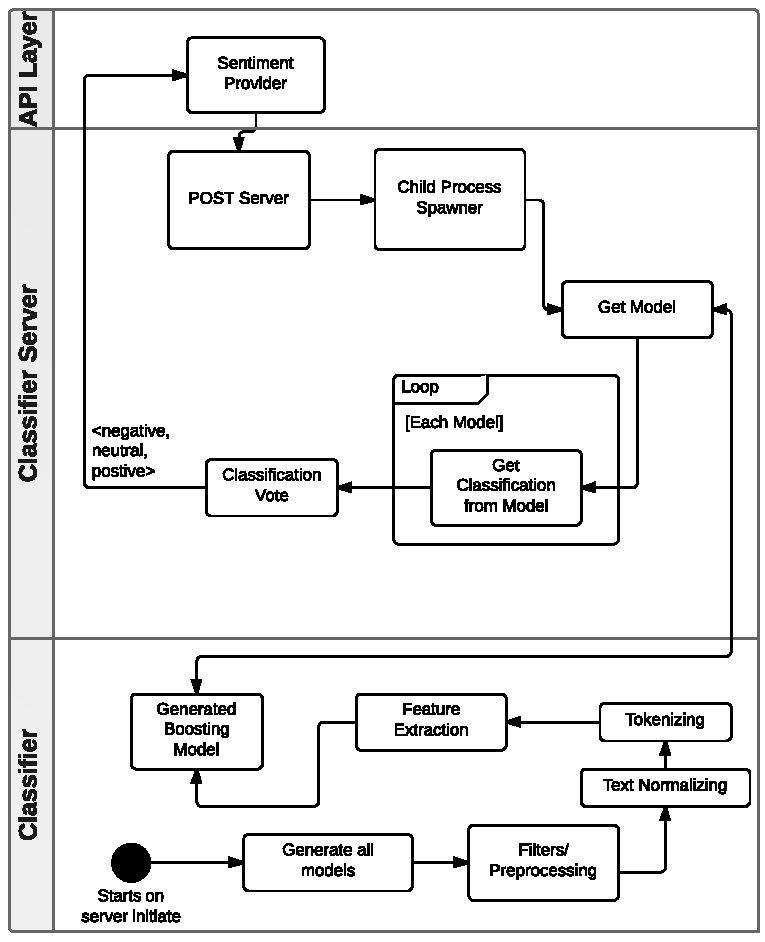
\includegraphics[width=0.8\textwidth]{../img/ClassifierArcitechture30Boosting.pdf}
 \end{center}
 \caption[Architectural overview of the classification server with Boosting.]{Architectural overview of the classification server with boosting. On server start, the Boosting model for predicting seniment is generated with a set of sub-models. When a request from the API Layer is made to the POST Server, a child processes is spawned. The tweet text is extracted and sent into the model for classification. All models predicts a sentiment and sends the sentiment to voting. For voting the Boosting model selects the sentiment with highest score and returns this to the API sentiment provider.}
 \label{fig:ClassifierArcitechtureBoosting}
\end{figure}

The Sentiment Provider module from the API Layer makes a request to the classifier's POST Server. The POST server translates the string to a Python dictionary and passes the information down to the Child Process Spawner. A new process is spawned and, using the module generated when initiating the server, the tweet is classified and returned to the API Layer.

When the classification model is trained on the server initialization, various text filters, normalizations and other pre-processing methods can be utilized, as seen in figure~\ref{fig:ClassifierArcitechture}. The model can be generated as either a one-step process, two-step process or a combination using Boosting. 

If a one-step model is used, one algorithm is used to classify the tweet as either negative, neutral or positive. If a two-step model is used, the tweet is first classified as either subjective or neutral in the subjectivity classification step. If it is neutral, the model returns with the classification. If the result is subjective, the tweet is sent to the polarity classification step, where the result can either be negative or positive. The end classification is returned to the API Layer.

When using the Boosting model, a set of sub-models is generated and all used in conjunction to predict a sentiment of a tweet. All sub-models predicts and sends the classification to a voting mechanism. The final classification is the result of the vote. This process is visualized in figure~\ref{fig:ClassifierArcitechtureBoosting}.

\subsubsection{Classification Model Structure}

The classification models are implemented by wrapping machine learning algorithms from sklearn in a inheritance based class structure. By having every model inherit from a base model, the interface is the same across every model, and the system can use the model without having knowledge what kind of algorithm it uses. An overview of this structure is presented in figure~\ref{fig:ModelsStructure}.

The base parent model implements methods for training the machine learning algorithm and for predicing either a set of documents or one document. For simple algorithms as NB, SVM and MaxEnt, these generic methods can be used, but the TwoStep and Boosting model have their own implementation. 
 
\begin{figure}[htb]
 \begin{center}
     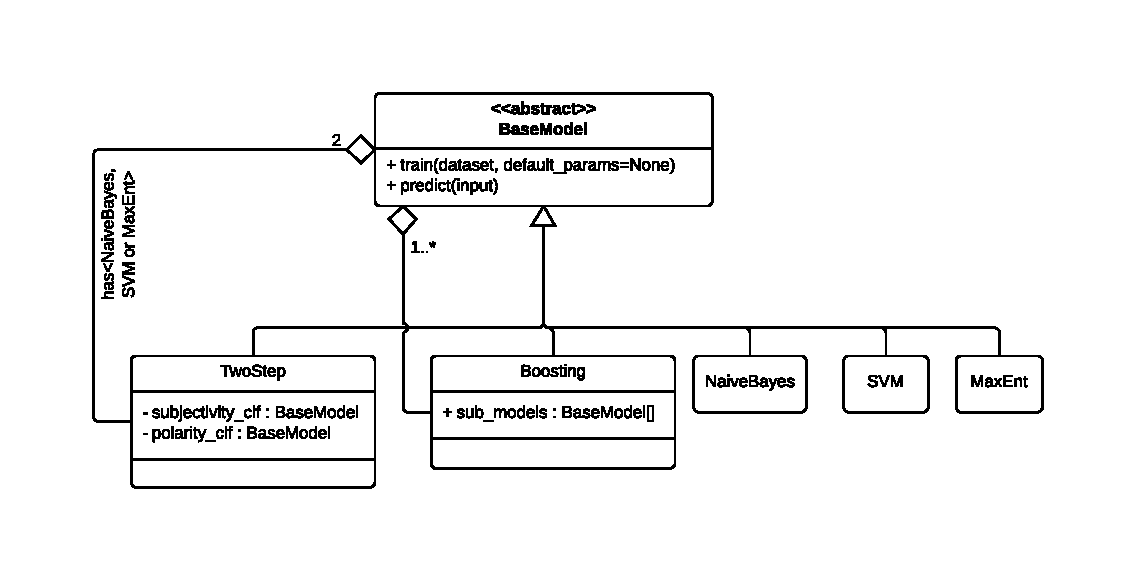
\includegraphics[width=0.8\textwidth]{../img/ModelsStructure.pdf}
 \end{center}
 \caption[Classification Model Structure Overview]{Overview of how the models are built and connected. There is a base model class implementing a method for predicing and training. All models extends from this base model. The models for NaiveBayes, SVM and MaxEnt uses the base model's implementation of train and predict, whilst the TwoStep and Boosting models implement their own. The interface for each model is the same.}
 \label{fig:ModelsStructure}
\end{figure}
